\section{Lecture 34}
\subsection{Lecture Notes - Course Review I}
\subsubsection{Quiz II Recap}
\phantom{i}
\begin{center}
    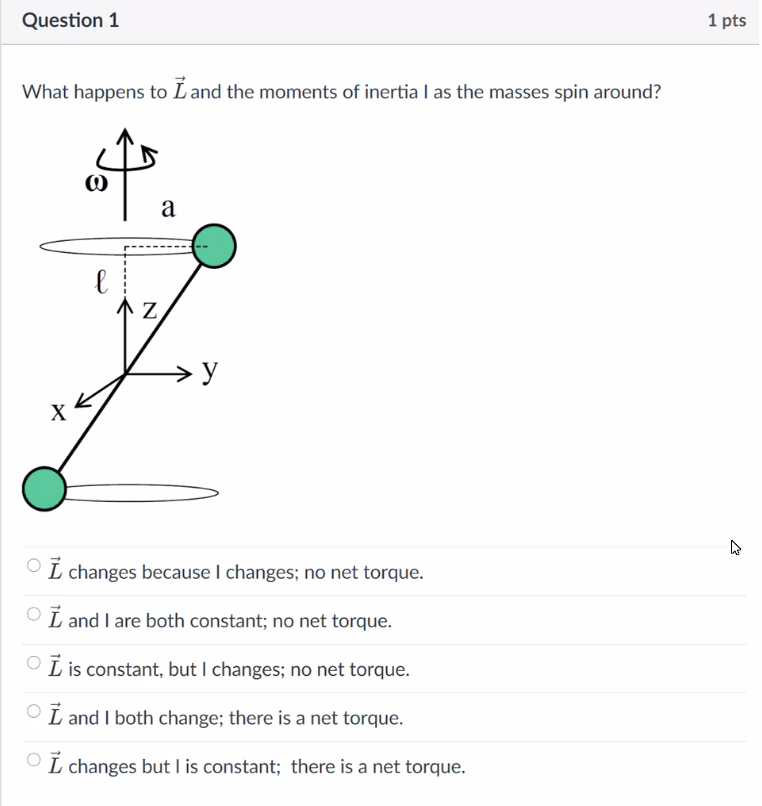
\includegraphics[scale=0.7]{Lecture-34/l34-img1.png}
\end{center}
\begin{s}
$\v{L}$ and and $\II$ both change; there is a net torque. $\v{L}$ is parallel to $\bm{\omega}$ when the rotation is about a principal axis, which is not the case here. Here, there are off diagonal elements in the inertia tensor. $\v{L}$ changes in time ($\v{r} \times \v{p}$ changes in time) and hence there must be a net torque $\bm{\Gamma}$ and the inertia tensor must change as well.
\end{s}
\begin{center}
    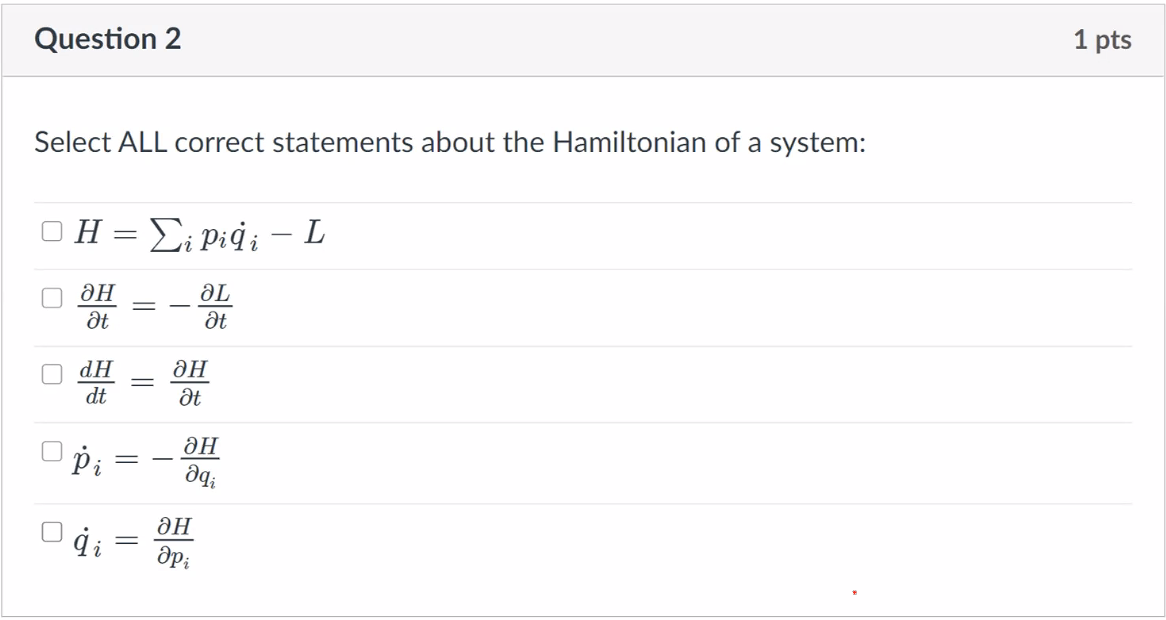
\includegraphics[scale=0.7]{Lecture-34/l34-img2.png}
\end{center}
\begin{s}
All of them! The first is the definition. The last two are Hamilton's equations. The last two are less obvious, but can be checked by differentiating the expression. Taking the derivative, we have:
\[\dod{\HH}{t} = \sum_i \dpd{\HH}{q_i}\dot{q}_i + \dpd{\HH}{p_i}\dot{p_i} + \dpd{\HH}{t}\]
Where the first two terms are zero by Hamilton's equations. We also have that:
\[\HH = \sum_i p_i\dot{q}_i(q, p, t) - \LL\]
So taking the derivative:
\[\dpd{\HH}{t} = p\dpd{\dot{q}}{t} - \dpd{\LL}{\dot{q}}\dpd{\dot{q}}{t} - \dpd{\LL}{t}\]
And the first two terms cancel using the Euler-Lagrange equation.
\end{s}
\begin{center}
    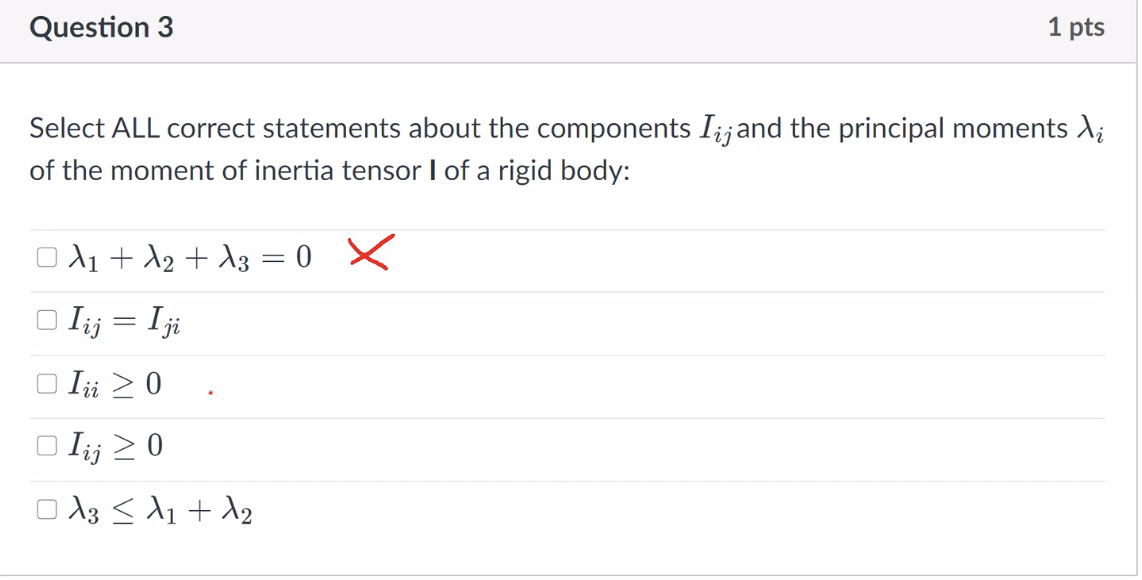
\includegraphics[scale=0.7]{Lecture-34/l34-img3.png}
\end{center}
\begin{s}
The first is false (no reason it should be!) The second is true as the moment of inertia tensor is symmetric by construction. The third is true by definition of the diagonal elements. The fourth is false. The last one is tricky:
\[\lambda_1 + \lambda_2 = \rho\int (x^2 + y^2)dV + 2\rho\int z^2 dV \geq \rho \int x^2 + y^2 dV = \lambda_3\]
\end{s}
\begin{center}
    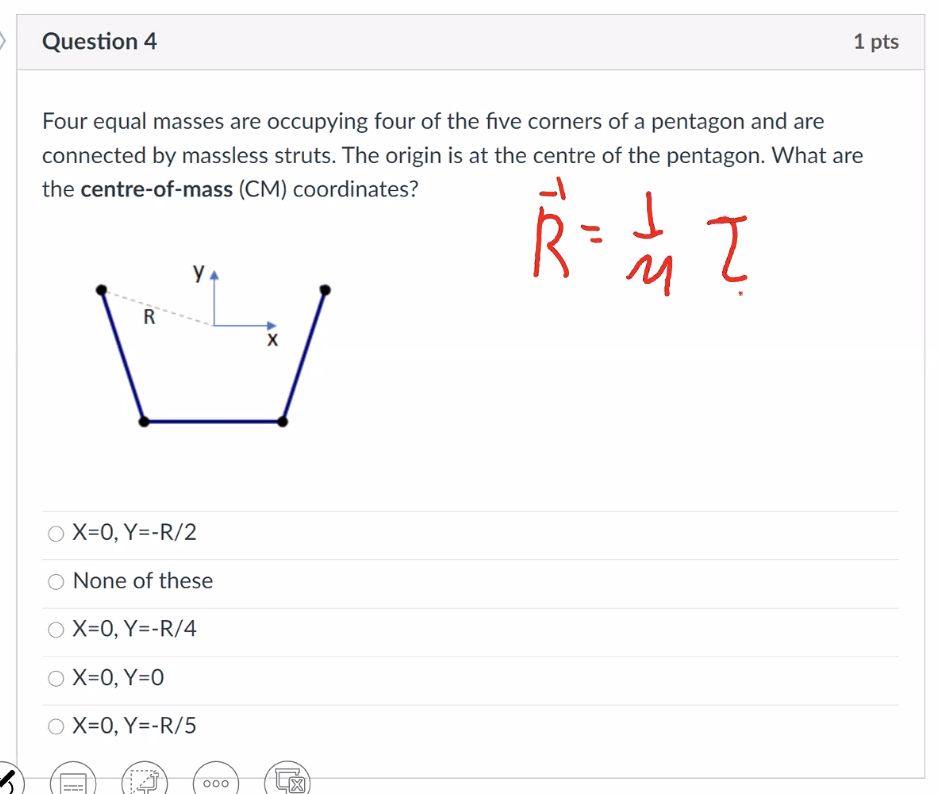
\includegraphics[scale=0.7]{Lecture-34/l34-img4.png}
\end{center}
\begin{s}
From the definition $\v{R} = \frac{1}{M}\sum_i \v{r}_im_i$, we see that the x component is immediately zero by symmetry. We could calculate the y component the pedestrian way by adding up all the contributions, or we can use a neat trick. If we complete the pentagon, then we have a center of mass at zero. Hence, we can imagine calculating the center of mass of the pentagon plus an "anti-mass" at the top vertex of the pentagon, which gives the easy result of $Y = -\frac{R}{4}$.
\end{s}

\begin{center}
    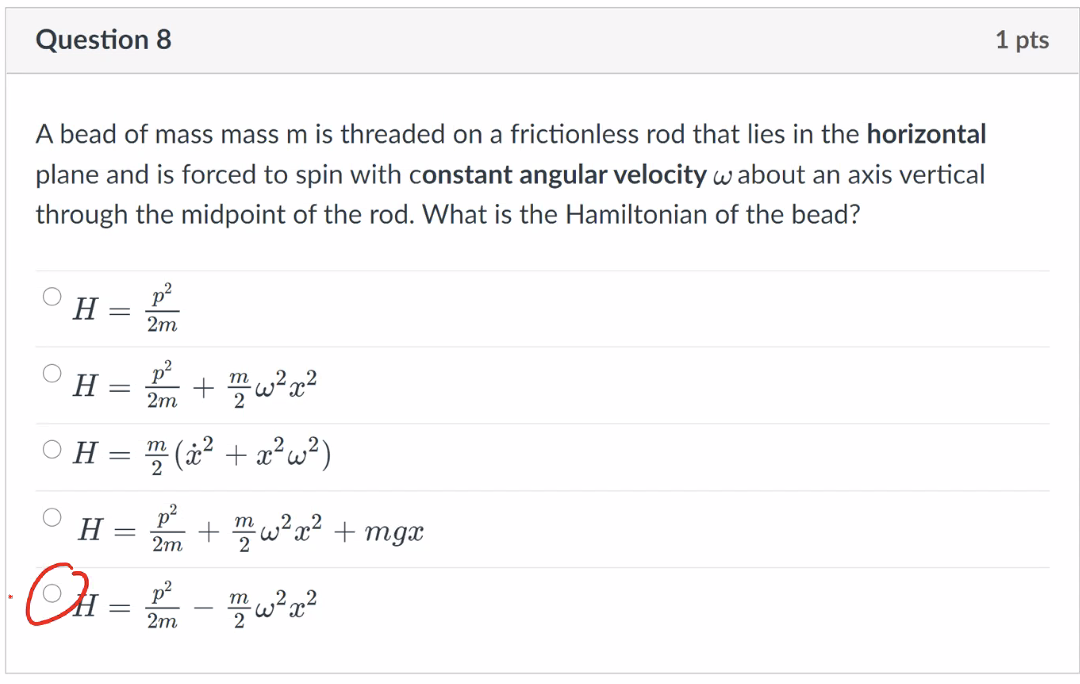
\includegraphics[scale=0.7]{Lecture-34/l34-img5.png}
\end{center}
\begin{s}
This question is somewhat deceptive; its tempting to use $\HH = T + U$, but this \textbf{does not hold} here, as the coordinate transformation is not natural. Hence, we have to return to the definition $\HH = \sum_i p_i\dot{q}_i - \LL$. Doing so, we realize the answer is:
\[\HH = \frac{p^2}{2m} - \frac{m}{2}\omega^2 x^2\]
Explicitly working it out step by step, we have that:
\[\LL = T - U = T = \frac{m}{2}(\dot{x}^@ + x^2\dot{\theta}^2) \]
There is no potential as we just rotate in a plane. Here we have that $\dot{\theta}^2 = \omega^2$, and in fact there is an explicit time dependence so the coordinate transformation is not natural. Hence:
\[\LL = \frac{m}{2}(\dot{x}^2 + x^2\omega^2)\]
And deriving $p$ we have that:
\[p = \dpd{\LL}{\dot{x}} = m\dot{x}\]
And furthermore:
\[dot{x} = \frac{p}{m}\]
Then, we have that the Hamiltonian is given by:
\[\HH = p\frac{p}{m} - \LL = \frac{p^2}{m} - \frac{1}{2}\frac{p^2}{m} - \frac{m}{2}x^2\omega^2 = \frac{m}{2}(\dot{x}^2 + x^2\omega^2)\]
\end{s}

\subsubsection{Euler Angles}
\begin{center}
    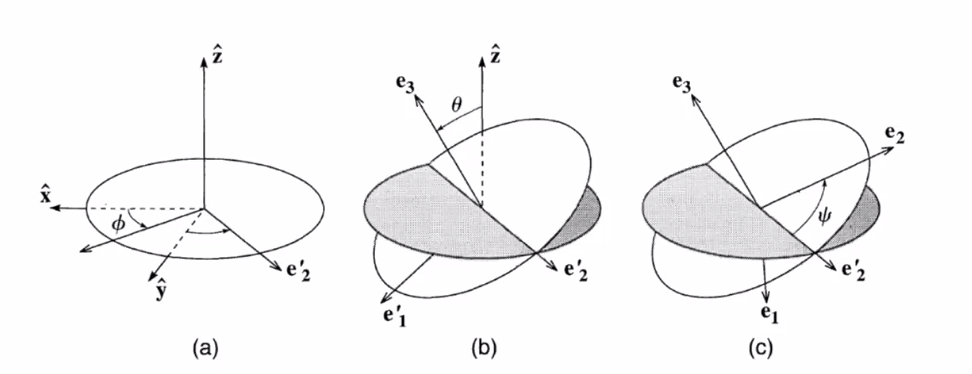
\includegraphics[scale=00.7]{Lecture-34/l34-img6.png}
\end{center}
\[
\begin{array}{c}
\mathbf{R}_{1}(\phi)=\left(\begin{array}{ccc}
\cos \phi & \sin \phi & 0 \\
-\sin \phi & \cos \phi & 0 \\
0 & 0 & 1
\end{array}\right) \\
\mathbf{R}_{2}(\theta)=\left(\begin{array}{ccc}
\cos \theta & 0 & -\sin \theta \\
0 & 1 & 0 \\
\sin \theta & 0 & \cos \theta
\end{array}\right) \\
\mathbf{R}_{3}(\psi)=\left(\begin{array}{ccc}
\cos \psi & \sin \psi & 0 \\
-\sin \psi & \cos \psi & 0 \\
0 & 0 & 1
\end{array}\right)
\end{array}
\]
This is the convention for successive rotations to obtain the orientation of a rigid body. The first step is a rotation by $\phi$ about the $\zhat$ axis. The second step is a rotation by angle $\theta$ about the new $\hat{\v{e}}'_2$ axis. Finally, we rotate by $\psi$ about the $\hat{\v{e}}_3$ axis. 
\subsubsection{Symmetric Top}
A classic application of the Euler angles is the symmetric top, where we want the angular momentum in the body frame. Using the rotations, we derived $\bm{\omega}$ in terms of the Euler angles and in terms of the unit vectors in the body frame:
\[
\vec{\omega}=(-\dot{\phi} \sin \theta \cos \psi+\dot{\theta} \sin \psi) \hat{\mathbf{e}}_{1}+(\dot{\phi} \sin \theta \sin \psi+\dot{\theta} \cos \psi) \hat{\mathbf{e}}_{2}+(\dot{\psi}+\dot{\phi} \cos \theta) \hat{\mathbf{e}}_{3}
\]
Using this, we found the kinetic energy:
\[
T=\frac{1}{2} \v{L} \cdot \bm{\omega}=\frac{1}{2}\left(\lambda_{1} \omega_{1}^{2}+\lambda_{2} \omega_{2}^{2}+\lambda_{3} \omega_{3}^{2}\right)
\]
Of course, the kinetic energy is the same whether calculated in the body frame or lab frame; the product of vectors is invariant of frame, though the vectors themselves may change. We then assumed $\lambda_1 = \lambda_2$ (symmetric top) and from this we derived the Lagrangian:
\[
\mathcal{L}=\frac{1}{2} \lambda_{1}\left(\dot{\phi}^{2} \sin ^{2} \theta+\dot{\theta}^{2}\right)+\frac{1}{2} \lambda_{3}(\dot{\psi}+\dot{\phi} \cos \theta)^{2}-M g R \cos \theta
\]
\subsubsection{What if the tip is free to slide?}
\begin{center}
    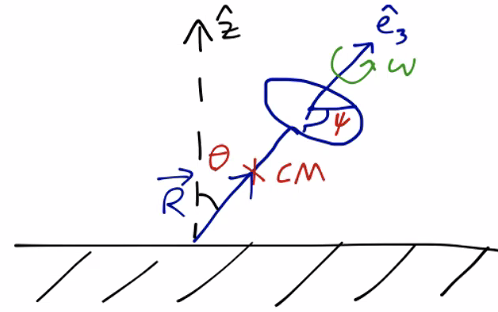
\includegraphics[scale=0.7]{Lecture-34/l34-img7.png}
\end{center}
If this is the case, then we modify the Lagrangian, using the fact that we can always decouple the translational and rotational motions of the rigid body:
\[\mathcal{L}=\frac{1}{2} M\left(\dot{X}^{2}+\dot{Y}^{2}+\dot{Z}^{2}\right)+\frac{1}{2} \lambda_{1}^{\mathrm{cm}}\left(\dot{\phi}^{2} \sin ^{2} \theta+\dot{\theta}^{2}\right)+\frac{1}{2} \lambda_{3}^{\mathrm{cm}}(\dot{\psi}+\dot{\phi} \cos \theta)^{2}-M g R \cos \theta\]
Which we see is just the kinetic energy of the COM $\frac{1}{2} M\left(\dot{X}^{2}+\dot{Y}^{2}+\dot{Z}^{2}\right)$ plus the rotational terms we determined earlier. If we have steady precession, then $\theta = \text{Const}$ and hence $\dot{z} = -R\sin\theta\dot{\theta} = 0$ (as $z = R\cos\theta$). One subtlety is we have to relate the center of mass moments to the moments when we had the tip fixed. Using the parallel axis theorem, we have that:
\[\lambda_1^{tip} = \lambda_1^{COM} + MR^2\]
\[\lambda_3^{tip} = \lambda_3^{COM}\]
So we can relate these terms very quickly. We recall the formula for the precession frequency:
\[\Omega = \frac{\lambda_3\omega_3}{\lambda_1\cos\theta}\]
In the case of free precession. In the two situations where the tip is fixed vs free, we consider:
\[\Omega^{tip} = \frac{\lambda_3^{tip}\omega_3}{\lambda_1^{tip}\cos\theta} < \Omega^{COM}\]
So it actually precesses slower if we let the tip freely move!

Next day, we will look at canonical transformations.